%!TEX root = ../main.tex
%chktex-file 17

\chapter{Evaluation}\label{sec:eval}

Due to the scarcity of similar tools, points of strong comparison for Gillian's
new debugger are few and far between. The best options to evaluate this project
against are the options available to Gillian users prior to this project (or
prior to any debugging work being done at all, as this project comes after
multiple years of work to this end), and to VeriFast, Gillian's closest
contemporary.

\section{Comparison: Previous Gillian Debugging Methods}

When compared to the previous debugging method---manually reading the (textual) log file
resulting from verification---the advantages of having a working visual debugger are evident. Not only does the log file require a deep understanding of Gillian's
internals, but it contains a vast amount of detail, often obfuscating the
information relevant to the encountered error. Moreover, the navigation from one point of interest to the next is highly non-trivial. 
Even in the simple case of the recursive list length function, which was used as
a baseline throughout the project, a total of 9328 lines of logging output is
generated during verification. As a more precise comparison, about 1500 of those
lines concern unification of the postconditions, with a high degree of
redundancy and verbosity. This contrasts with what is essentially a few lines of
text in the debugger interface, with more detail available as and when the user
requires. Compared to the clear, clean, and concise interface of the new
solution, a far more ideal debugging process has been presented---even those
with a deep understanding of Gillian, who are well acclimated to debugging via
the file log, intend to use this as their primary method of debugging moving
forwards.

\todo{Add a specific example --- reference background?}

The new debugger also brings substantial improvement when compared to the previous iterations: aside from not having any unification information whatsoever, their use required of the user to understand the quirks of the solution, such as branches being executed one after the other with no means of discerning between then. 
The iterations of the debugger were very much a case of attempting to move Gillian a step closer to debugging in whatever manner was available, rather than setting out a clear vision of what prospective users would desire from a program verification debugger, and working to meet that goal.

\section{Vs. VeriFast}

VeriFast has a fundamentally different approach to the debugging process;
instead of reporting the results of symbolic execution step by step, the whole
verification is performed all at once, only showing details in the event of an
error (or a breakpoint being reached). There is no concept of exploring the
different execution paths of the program, severely limiting its ability to be
used as a tool for deepening one's understanding of the underlying reasoning. Multiple
branches of execution are not presented to the user, only showing the single
path taken to reach the error or breakpoint. This textual format is far more rigid than the Gillian debugger's explorable execution map given in
\autoref{fig:verifast-path-compare}; not only is the latter more feature-rich,
but it also provides a complete overview of the program execution.

\begin{figure}
  \centering
  \begin{subfigure}[b]{0.4\textwidth}
    \center{}
    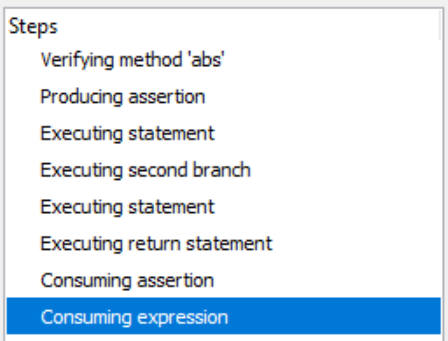
\includegraphics[width=0.75\textwidth]{img/verifast-path.png}
    %\caption{The execution path information given by VeriFast}%
    %\label{fig:verifast-path}
  \end{subfigure}
  \qquad
  \begin{subfigure}[b]{0.4\textwidth}
    \centering
    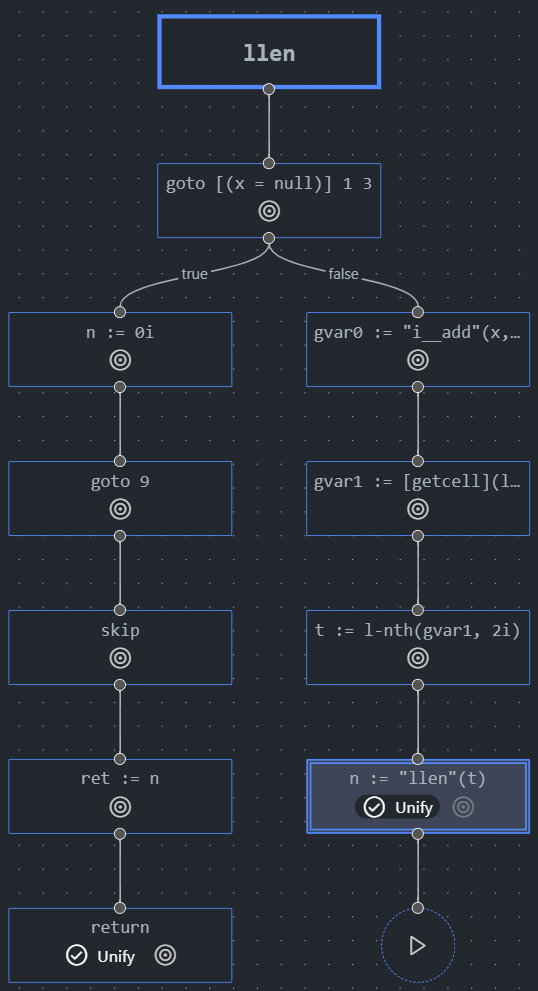
\includegraphics[width=0.9\textwidth]{img/execmap-final.png}
    %\caption{The Gillian debugger's execution map}%
    %\label{fig:execmap-final}
  \end{subfigure}
  \caption{Execution Path/Branching Information: VeriFast (left); (b) the Gillian
  debugger (right)}%
  \label{fig:verifast-path-compare}
\end{figure}

VeriFast also gives no insight into the unification process; the only
information provided is an error message should unification fail. The Gillian
debugger gives more information to this end by showing all assertions from
a unification, up to and including the failing one, as shown in \autoref{fig:verifast-path-compare}.

\begin{figure}
  \centering
  \begin{subfigure}[b]{0.4\textwidth}
    \center{}
    
\includegraphics[width=0.9\textwidth]{img/verifast-error.png}
    %\caption{A unification error given by VeriFast}%
    %\label{fig:verifast-error}
  \end{subfigure}
  \qquad
  \begin{subfigure}[b]{0.4\textwidth}
    \centering
    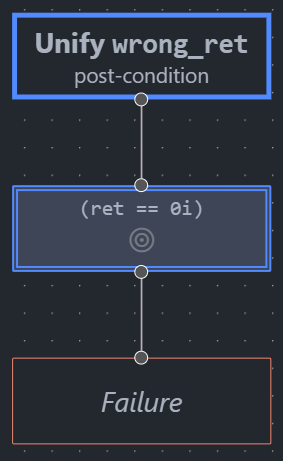
\includegraphics[width=0.3\textwidth]{img/unifymap-failure.png}
    %\caption{A failing unification map given by the Gillian debugger}%
    %\label{fig:unifymap-failure}
  \end{subfigure}
  \caption{Failing Unification Information: Verifast (left); (b) Gillian debugger (right)}%
  \label{fig:verifast-unifyfail-compare}
\end{figure}

Another point of comparison is the accessibility of the different solutions.
VeriFast is a completely isolated tool, its graphical interface needing to be
run separately from any other software used for development. Now, armed with the
new debugging functionality, developers have a real possibility of using Gillian
as part of their development pipeline; the ability to debug Gillian verification
directly inside VSCode (by far the most popular editor in the world) is, we believe, a
previously unmatched level of accessibility for a tool of this purpose.

\sacha{You probably need concrete examples of debugging programs with bugs. And also, a concrete example of a BIG program (i.e. amazon-c string bug for example, non-lifted)}

\section{Limitations}%
\label{sec:eval:limitations}

Although this project has made substantial progress towards making Gillian a more
user-friendly and mainstream tool, there are still several limitations that need to be
addressed.

\myparagraph{Incomplete target language lifting.}
As discovered in \autoref{sec:debug-interface}, the mechanism to lift the
debugging process to the level of the target language is currently incomplete,
due to particular mechanisms of how multiple GIL commands are coalesced back
into a single target language command, preventing full support for lifting
execution maps to represent the target language.
Thankfully, these issues are very low-hanging fruit. However, the challenges
involved in supporting lifting for more of the verification process could
constitute another entire Masters project on their own, such as lifting the symbolic
state, and various kinds of errors, to a point where no knowledge of GIL would
be required to debug the verification of a program written in a supported target
language (for example, JavaScript).

\myparagraph{Lack of annotations on the GIL AST.}
The current debugger highlights which part of the code is being symbolically
executed; however, there is no such mechanism during unification.
For example, the debugger does not highlight what part of the state is being
affected by a particular assertion. The addition of state highlighting, or even
highlighting previous parts of code that were the last to affect parts of the
state, would do much to create a more intuitive connection between the code and
the unification process.

\myparagraph{Performance.}
Logging in Gillian is quite slow. In the past, the creators of Gillian put much
effort into minimising the overhead of the logging infrastructure when logging
is disabled. Executing verification and logging into a file (the old way) is
about 5.75\footnotemark[1]{} times slower than executing verification with
logging disabled. In the new infrastructure, executing verification and logging
to the database is 2.32\footnotemark[1]{} times slower than when logging into
the file, thus 13.35\footnotemark[1]{} times slower than no logging at all.
For small WISL programs, such as those studied in the Separation Logic course,
programs are simple enough for this time difference to be negligible. However,
full verification of the fragment of the \texttt{AWS Encryption SDK} takes about
6 minutes on a modern high-end laptop, meaning the relative performance of the
debugger would be far too sluggish for mainstream use. \footnotetext[1]{Measures
performed on the available benchmark for WISL verification.} That being said,
our expertise gives us confidence that these performance numbers can be
greatly improved upon with a relatively small amount of work.
The two most obvious improvements are \textbf{(1)} making the database
interaction asynchronous (or potentially multithreaded), and \textbf{(2)}
finding a more efficient method of serialising data than JSON---perhaps
Protocol Buffers~\cite{protobuf}. Interestingly, implementing \textbf{(1)} may
result in database logging becoming more efficient than logging into a file,
since file-logging must be performed synchronously as to preserve the order of
the logs, while records can be written in any order in the database while
preserving the necessary structure.

\paragraph{Tool-developer experience.}
However powerful the logging structure is, its API is far from perfect at
present. Retrieving previously logged data from the database requires writing
SQL queries by hand, followed by calling the OCaml-SQL driver. However, given
the principled structure of the log trace, this experience could be largely
improved by designing a domain-specific query language adapted to extracting any
kind of information from the traces. Note, however, that this limitation only
affects the tool developer, and does not affect the primary customer of this
project, the tool user.

Of course, none of these factors detract from the fact that, from the
perspective of user experience, this project has elevated Gillian from a
prototype research tool to one that that proves useful in pursuing new research
in program analysis, and even more importantly, a tool that can be used for
educational purposes---to help those having their first experience of
program analysis, separation logic, and symbolic execution form a deeper understanding by automatically applying its
principles to actual programs.
